%% AMS-LaTeX Created with the Wolfram Language for Students - Personal Use Only : www.wolfram.com

\documentclass{article}
\usepackage{amsmath, amssymb, graphics, setspace}

\newcommand{\mathsym}[1]{{}}
\newcommand{\unicode}[1]{{}}

\newcounter{mathematicapage}
\begin{document}

\section*{Reactions}

\subsection*{Exercise 4.C1}

The plan here is to abstract the reaction solver, to *hopefully* solve a system of reactions, by invoking equilibrium (assuming statically determinate;
though I suppose that statically indeterminate will just return no solution.)\\
\\
To this we abstract every force to a magnitude, direction, and location.

\begin{doublespace}
\noindent\(\pmb{\text{fArbitrary}=\{\text{{``}Label{''}}, \text{fArbMag}, \{\text{dx}, \text{dy}, \text{dz}\}, \{\text{cx},\text{cy},\text{cz}\}\}}\)
\end{doublespace}

\begin{doublespace}
\noindent\(\{\text{Label},\text{fArbMag},\{\text{dx},\text{dy},\text{dz}\},\{\text{cx},\text{cy},\text{cz}\}\}\)
\end{doublespace}

Now the problem:

We first make a list of all of the forces. We can immediately get the equations for the sum of the forces (in x and y) and the sum of the moments
about the origin (point A in this case).

\begin{doublespace}
\noindent\(\pmb{\text{Clear}[\text{tMag},\text{aXMag},\text{AYMag},\text{theta}]}\\
\pmb{\text{forceList4C1}=\{}\\
\pmb{\{\text{{``}PLoad{''}},\text{Quantity}[50,\text{{``}Pounds{''}}],\{0,-1,0\},}\\
\pmb{\text{Simplify}[\{27*\text{Sin}[\text{theta}]+4*\text{Cos}[\text{theta}],-27*\text{Cos}[\text{theta}]+4*\text{Sin}[\text{theta}],0\}]\},}\\
\pmb{\{\text{{``}Tension E{''}},\text{tMag},\text{Normalize}[\{8-12*\text{Sin}[\text{theta}],16+12*\text{Cos}[\text{theta}],0\}],}\\
\pmb{\{12*\text{Sin}[\text{theta}],-12*\text{Cos}[\text{theta}],0\}\},}\\
\pmb{\text{(*}\{\text{{``}Tension E{''}},\text{tMag},\{0,1,0\},\{12*\text{Sin}[\text{theta}],-12*\text{Cos}[\text{theta}],0\}\},\text{*)}}\\
\pmb{\{\text{{``}Ax Reaction{''}},\text{aXMag},\{1,0,0\},\{0,0,0\}\},}\\
\pmb{\{\text{{``}Ay Reaction{''}},\text{aYMag},\{0,1,0\},\{0,0,0\}\} \text{(*},}\\
\pmb{\{\text{{``}Gravity Bar{''}},\text{gravMag},\{\text{dGx},\text{dGy},0\},\{27*\text{Sin}[\text{theta}],27*\text{Cos}[\text{theta}],0\}\}\text{*)}}\\
\pmb{\};}\\
\pmb{}\\
\pmb{\text{numForces}=\text{Length}[\text{forceList4C1}];}\\
\pmb{\text{forceNet}=\text{Sum}[\text{forceList4C1}[[i]][[2]]*\text{forceList4C1}[[i]][[3]],\{i,1,\text{numForces}\}]}\\
\pmb{\text{momentNet}= }\\
\pmb{\text{Sum}[\text{forceList4C1}[[i]][[2]]*((\text{forceList4C1}[[i]][[4]])\times \text{forceList4C1}[[i]][[3]]),}\\
\pmb{\{i,1,\text{numForces}\}]}\)
\end{doublespace}

\begin{doublespace}
\noindent\(\left\{\text{aXMag}++\frac{\text{tMag} (8-12 \text{Sin}[\text{theta}])}{\sqrt{\text{Abs}[16+12 \text{Cos}[\text{theta}]]^2+\text{Abs}[8-12
\text{Sin}[\text{theta}]]^2}},\text{aYMag}+\frac{\text{tMag} (16+12 \text{Cos}[\text{theta}])}{\sqrt{\text{Abs}[16+12 \text{Cos}[\text{theta}]]^2+\text{Abs}[8-12
\text{Sin}[\text{theta}]]^2}}+,\right\}\)
\end{doublespace}

\begin{doublespace}
\noindent\(\left\{,,() (-4 \text{Cos}[\text{theta}]-27 \text{Sin}[\text{theta}])+\text{tMag} \left(\frac{96 \text{Cos}[\text{theta}]}{\sqrt{\text{Abs}[16+12
\text{Cos}[\text{theta}]]^2+\text{Abs}[8-12 \text{Sin}[\text{theta}]]^2}}+\frac{192 \text{Sin}[\text{theta}]}{\sqrt{\text{Abs}[16+12 \text{Cos}[\text{theta}]]^2+\text{Abs}[8-12
\text{Sin}[\text{theta}]]^2}}\right)\right\}\)
\end{doublespace}

Invoking Equilibrium, sum of forces and sum of moments equal the zero vectors

\begin{doublespace}
\noindent\(\pmb{\text{StringForm}[\text{{``}Invoking Equilibrium, sum of forces and sum of moments{''}}]}\\
\pmb{\text{Solve}[\text{forceNet}==\{0,0,0\},\{\text{aXMag},\text{aYMag}\}]}\\
\pmb{\text{Solve}[\text{momentNet}==\{0,0,0\},\{\text{tMag}\}]}\\
\pmb{}\\
\pmb{\text{StringForm}[\text{{``}Converting to a table{''}}]}\\
\pmb{\text{sol4C1Flat}=\text{Table}[}\\
\pmb{\text{Flatten}[}\\
\pmb{\left\{\text{theta}*\frac{180}{\pi },\{\text{tMag},\text{aXMag},\text{aYMag}\}\text{/.}\right.}\\
\pmb{\text{Solve}[\text{forceNet}==\{0,0,0\}\&\&\text{momentNet}==\{0,0,0\},\{\text{tMag},\text{aXMag},\text{aYMag}\}]\}],}\\
\pmb{\left.\left\{\text{theta},0,120*\frac{\pi }{180},10*\frac{\pi }{180}\right\}\right];}\\
\pmb{N[\text{sol4C1Flat}]}\)
\end{doublespace}

\begin{doublespace}
\noindent\(\text{Invoking Equilibrium, sum of forces and sum of moments}\)
\end{doublespace}

\begin{doublespace}
\noindent\(\left\{\left\{\text{aXMag}\to -\frac{8 \text{tMag}}{\sqrt{\text{Abs}[16+12 \text{Cos}[\text{theta}]]^2+\text{Abs}[8-12 \text{Sin}[\text{theta}]]^2}}+\frac{12
\text{tMag} \text{Sin}[\text{theta}]}{\sqrt{\text{Abs}[16+12 \text{Cos}[\text{theta}]]^2+\text{Abs}[8-12 \text{Sin}[\text{theta}]]^2}},\text{aYMag}\to
-\frac{16 \text{tMag}}{\sqrt{\text{Abs}[16+12 \text{Cos}[\text{theta}]]^2+\text{Abs}[8-12 \text{Sin}[\text{theta}]]^2}}-\frac{12 \text{tMag} \text{Cos}[\text{theta}]}{\sqrt{\text{Abs}[16+12
\text{Cos}[\text{theta}]]^2+\text{Abs}[8-12 \text{Sin}[\text{theta}]]^2}}+\right\}\right\}\)
\end{doublespace}

\begin{doublespace}
\noindent\(\left\{\left\{\text{tMag}\to \frac{\sqrt{\text{Abs}[16+12 \text{Cos}[\text{theta}]]^2+\text{Abs}[8-12 \text{Sin}[\text{theta}]]^2} \left(\right)
(4 \text{Cos}[\text{theta}]+27 \text{Sin}[\text{theta}])}{\text{Cos}[\text{theta}]+2 \text{Sin}[\text{theta}]}\right\}\right\}\)
\end{doublespace}

\begin{doublespace}
\noindent\(\text{Converting to a table}\)
\end{doublespace}

\begin{doublespace}
\noindent\(\{\{0.,,,\},\{10.,,,\},\{20.,,,\},\{30.,,,\},\{40.,,,\},\{50.,,,\},\{60.,,,\},\{70.,,,\},\{80.,,,\},\{90.,,,\},\{100.,,,\},\{110.,,,\},\{120.,,,\}\}\)
\end{doublespace}

We separate the values into different lists and plot the result

\begin{doublespace}
\noindent\(\pmb{\text{thetaDegVals}=\text{sol4C1Flat}[[1\text{;;},1]];}\\
\pmb{\text{tMagVals}=\text{sol4C1Flat}[[1\text{;;},2]];}\\
\pmb{\text{aXMagVals}=N[\text{sol4C1Flat}[[1\text{;;},3]]];}\\
\pmb{\text{aYMagVals}=N[\text{sol4C1Flat}[[1\text{;;},4]]];}\\
\pmb{\text{thetaCrit}=\text{ArcSin}\left[\frac{8}{12}\right]*\frac{180}{\pi };}\\
\pmb{N[\text{thetaCrit}]}\\
\pmb{\text{ListLinePlot}[\text{Flatten}[\{\text{thetaDegVals},\text{tMagVals}\},\{\{2\},\{1\}\}],}\\
\pmb{\text{AxesLabel}\to \{\text{{``}Angle from Vertical{''}},\text{{``}Tension force{''}}\},\text{PlotRange}\to \text{All}, }\\
\pmb{\text{PlotMarkers}\to \{\text{Automatic}, 10\}]}\)
\end{doublespace}

\begin{doublespace}
\noindent\(41.8103\)
\end{doublespace}

%$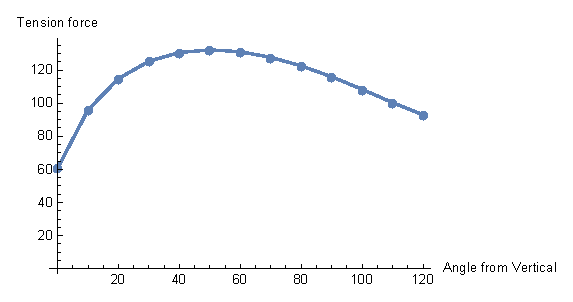
\includegraphics{02 - Reactions2_gr1.eps}$

To check our angles, we can plot the location of the tension force and the load. (It follows the bar movement as a function of theta.

\begin{doublespace}
\noindent\(\pmb{\text{endofLrod}=}\\
\pmb{N\left[\text{Table}\left[\left\{\text{theta}*\frac{180}{\pi },27*\text{Sin}[\text{theta}]+4*\text{Cos}[\text{theta}],-27*\text{Cos}[\text{theta}]+4*\text{Sin}[\text{theta}]\right\},\right.\right.}\\
\pmb{\left.\left.\left\{\text{theta},0,120*\frac{\pi }{180},10*\frac{\pi }{180}\right\}\right]\right]}\\
\pmb{\text{endofLrod}[[1\text{;;},2\text{;;}3]];}\\
\pmb{\text{midofRod}=}\\
\pmb{N\left[\text{Table}\left[\left\{\text{theta}*\frac{180}{\pi },12*\text{Sin}[\text{theta}], -12*\text{Cos}[\text{theta}]\right\},\left\{\text{theta},0,120*\frac{\pi
}{180},10*\frac{\pi }{180}\right\}\right]\right];}\\
\pmb{\text{ListPlot}[\{\text{endofLrod}[[1\text{;;},2\text{;;}3]],\text{midofRod}[[1\text{;;},2\text{;;}3]]\},\text{AspectRatio}\to \text{Automatic},}\\
\pmb{\text{AxesLabel}\to \{\text{{``}X Direction{''}},\text{{``}Y Direction{''}}\}, \text{PlotMarkers}\to \{\text{Automatic}, 10\}]}\)
\end{doublespace}

\begin{doublespace}
\noindent\(\{\{0.,4.,-27.\},\{10.,8.62773,-25.8952\},\{20.,12.9933,-24.0036\},\{30.,16.9641,-21.3827\},\{40.,20.4194,-18.112\},\{50.,23.2544,-14.2911\},\{60.,25.3827,-10.0359\},\{70.,26.7398,-5.47577\},\{80.,27.2844,-0.74927\},\{90.,27.,4.\},\{100.,25.8952,8.62773\},\{110.,24.0036,12.9933\},\{120.,21.3827,16.9641\}\}\)
\end{doublespace}

%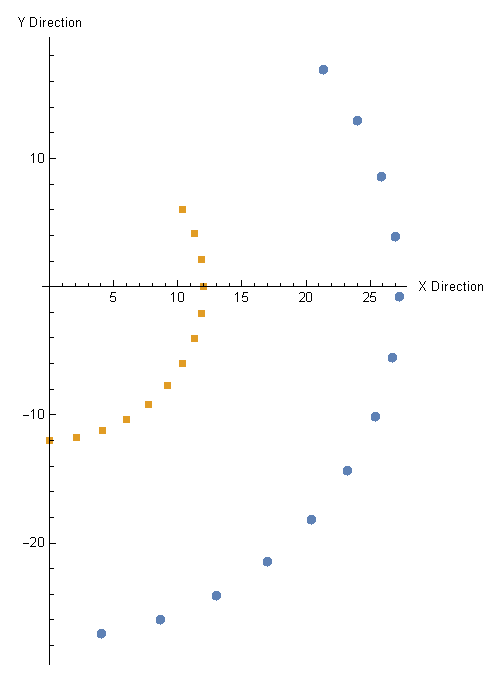
\includegraphics{02 - Reactions2_gr2.eps}

\end{document}
